\chapter{Grid HTM}
\label{sec:grid_htm}
\section{Introduction}
When it comes to applying \gls*{htm} on videos, this thesis proposes to use segmentation techniques to simplify the data into an SDR-friendly format. These segmentation techniques could be everything from simple binary thresholding to deep learning instance segmentation. Even keypoint detectors such as ORB\cite{orb_detector} could be applied. When explaining Grid HTM, the examples will be taken from deep learning instance segmentation of cars on a video from the VIRAT \cite{VIRAT} dataset.
\begin{figure}[H]
    \centering
    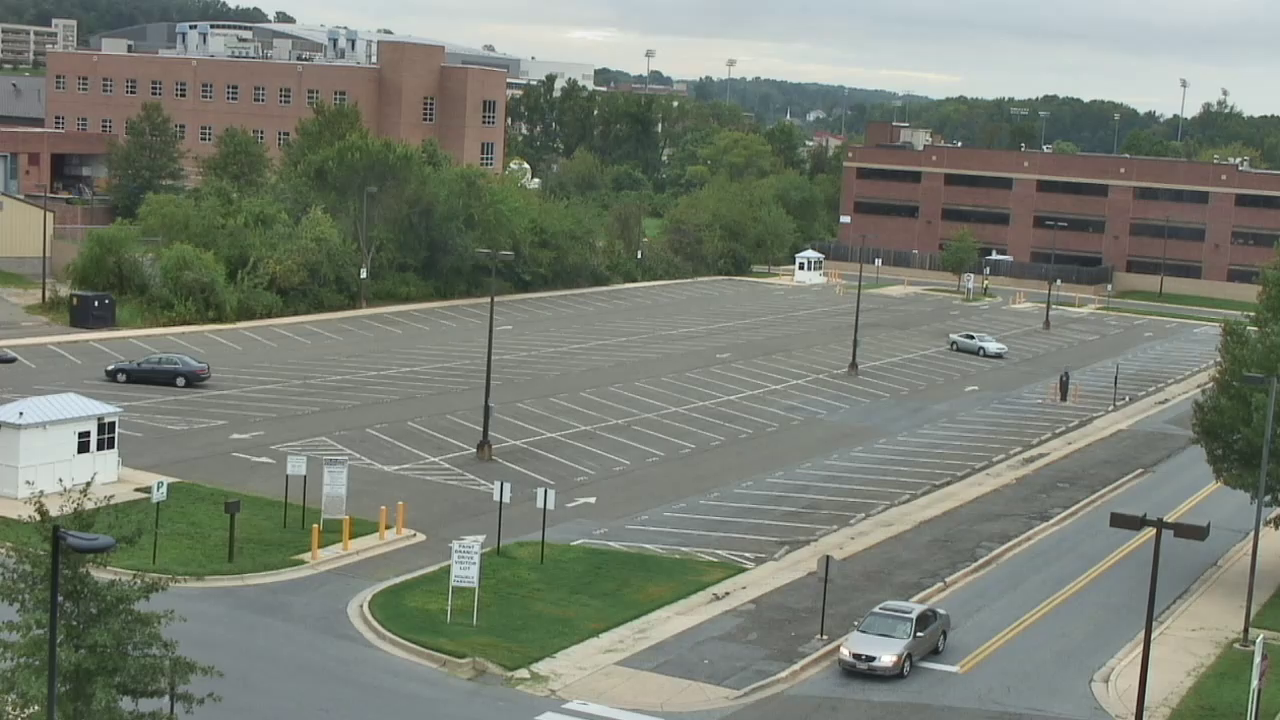
\includegraphics[width=.45\textwidth]{resources/methodology/original.png}
    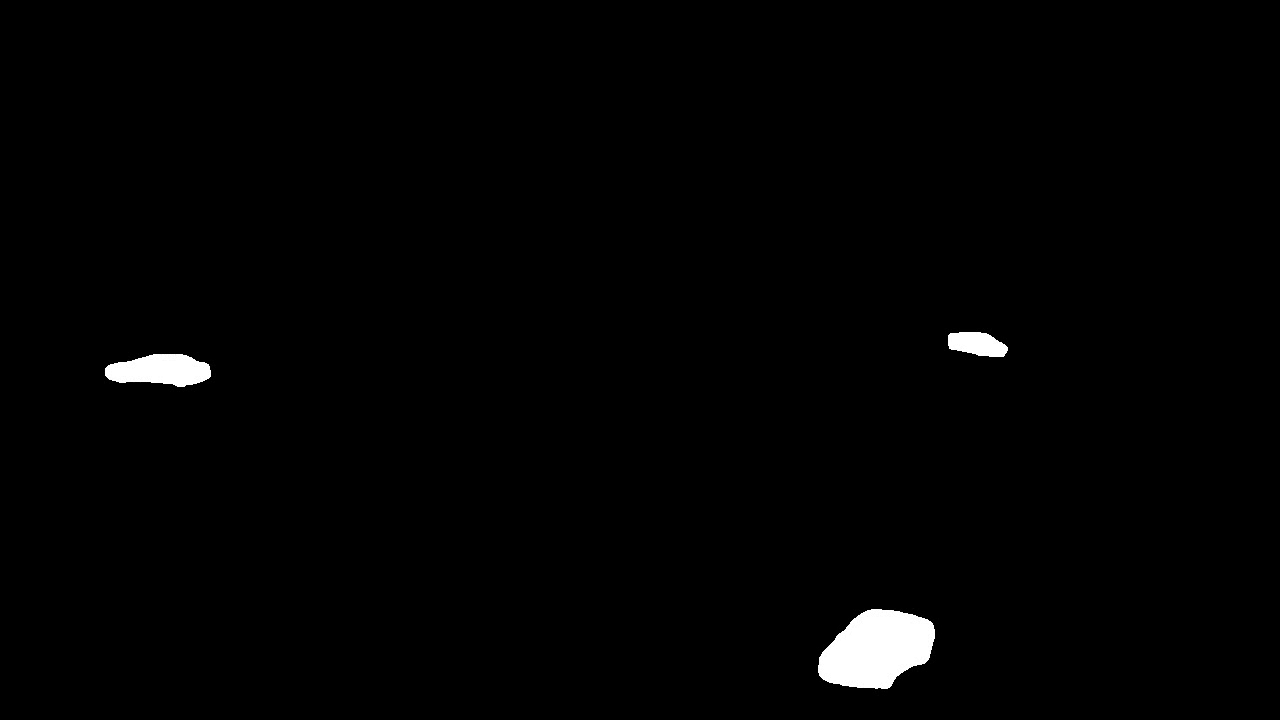
\includegraphics[width=.45\textwidth]{resources/methodology/car_segmentation.png}
    \caption{Segmentation result of cars, which is suited to be used as an SDR. Original frame taken from \cite{VIRAT}.}
\end{figure}
The idea is that the \gls*{sp} will learn to find an optimal general representation of cars. How general this representation is can be configured using the various parameters, but ideally they should be set so that different cars will be represented similarly while trucks and motorcycles will be represented differently.
\begin{figure}[H]
    \centering
    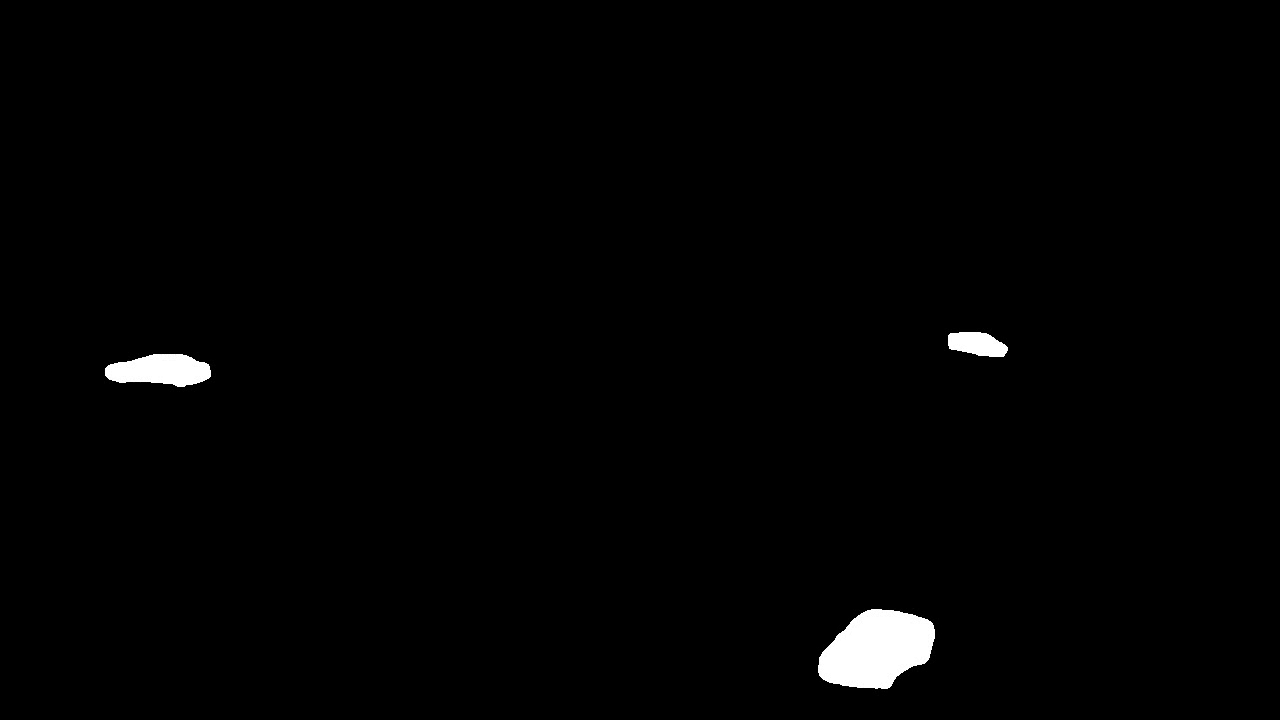
\includegraphics[width=.48\textwidth]{resources/methodology/car_segmentation.png}
    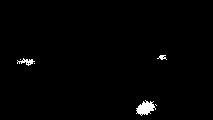
\includegraphics[width=.48\textwidth]{resources/methodology/car_segmentation_sp.png}
    \caption{The SDR and its corresponding \gls*{sp} representation. Note that the \gls*{sp} is untrained.}
\end{figure}
\par
The task of the \gls*{tm} will then be to learn the common patterns that the cars exhibit, their speed, shape, and positioning will be taken into account. Finally, the learning will be set so that new patterns are learned quickly, but forgotten slowly. This will allow the system to quickly learn the norm, even if there is little activity, while still reacting to anomalies. This requires that the input is stationary, in our example this means that the camera is not moving.
\par
Ideally, the system will have a calibration period spanning several days or weeks, during which the system is not performing any anomaly detection, but is just learning the patterns.\par
\section{Improvements}
\subsection{Invariance and Explainability}
One issue that becomes evident is the lack of invariance. Because the \gls*{tm} is learning the global patterns, in our example it learns that it is normal for cars to drive along the road but only in the context of there being cars parked in the parking lot. It is instead desired that the \gls*{tm} learns that it is normal for cars to drive along the road, regardless of whether there are cars in the parking lot. This thesis proposes a solution based on dividing the encoder output into a grid, and have a separate \gls*{sp} and \gls*{tm} for each cell in the grid. The anomaly scores of all the cells are then aggregated into a single anomaly score using an aggregation function.
\begin{figure}[H]
    \centering
    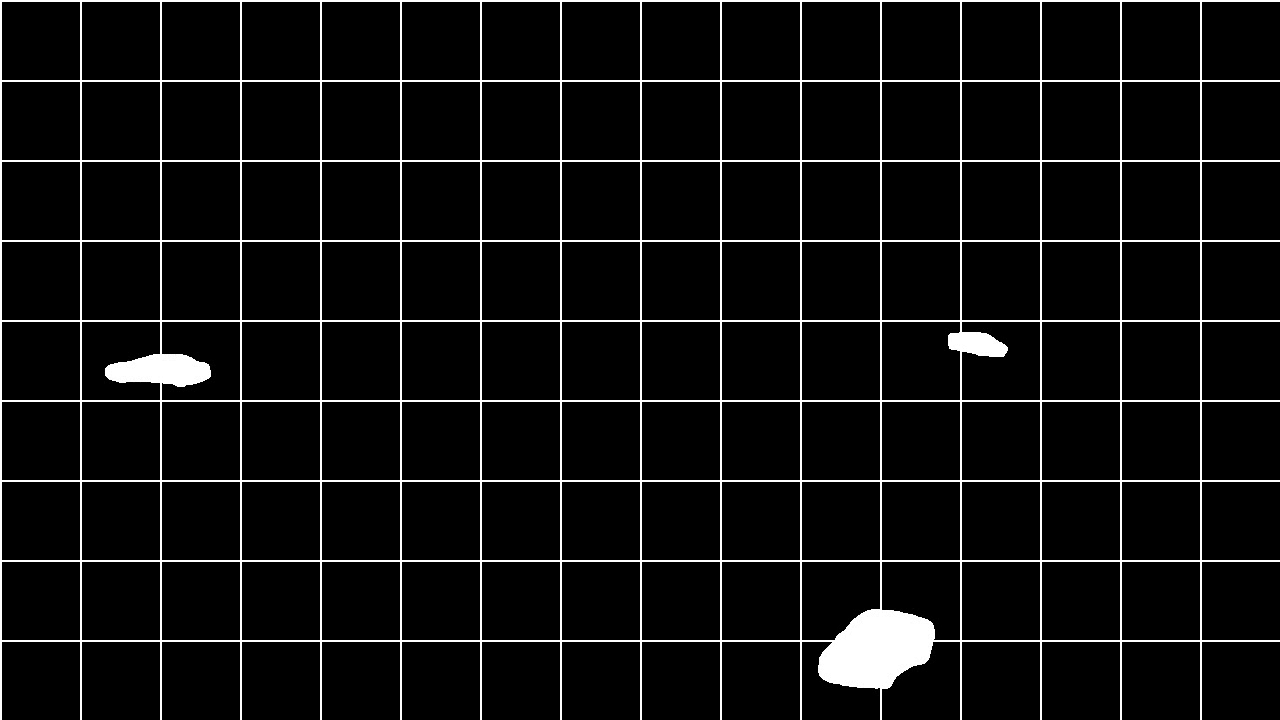
\includegraphics[width=\textwidth]{resources/methodology/car_segmentation_grid.png}
    \caption{The encoder output divided into a grid.}
    \label{fig:grid}
\end{figure}
It might be tempting to use the mean of all the anomaly scores as the aggregation function, but this leads to problems with normalization, meaning that an overall anomaly score of 1 is hard to achieve due to many cells having a zero anomaly score. In fact, it becomes unclear what a high anomaly score is anymore.
\par
An example is that one cell with a high anomaly score will lead to the same average anomaly score as every cell having a small anomaly score. That being said, the selection of an aggregation function depends on how noisy the input data is. For data with little noise, a potential aggregation function could be the non-zero mean:
\begin{align*}
    X         & :\{x : x > 0\} \\
    anomScore & =
    \begin{cases}
        \frac{\sum_{x \in X}x}{|X|} & \text{if } |X| > 0 \\
        0                           & \text{else}
    \end{cases}
\end{align*}
Meaning that only the cells with a non-zero anomaly score will be contributing to the overall anomaly score, which helps solve the aforementioned normalization problem. On the other hand, this will perform poorly when the system is exposed to noisy data which could lead to there always being a cell somewhere with a high anomaly score.

Having the encoder output divided into a grid has the added benefit of introducing explainability into the model. By using Grid \gls*{htm} it is now possible to find out where in the input an anomaly has occurred. Combined with the ability to estimate the number of predictions at any given time for any cell, makes this an attractive approach. In addition, it is also possible to configure the \gls*{sp} and the \gls*{tm} in each cell independently, giving the system increased flexibility. Last but not least, dividing it into smaller cells makes it possible to run each cell in parallel for increased performance.
\subsection{Reviewing Encoder Rules}
That being said, a potential problem with this approach is that the previously mentioned rules for creating a good encoder may not be respected, and therefore should be reviewed:
\begin{itemize}
    \item \textbf{Semantically similar data should result in SDRs with overlapping active bits}. In this example, a car at one position will produce an SDR with a high amount of overlapping bits as another car at a similar position in the input image.
    \item \textbf{The same input should always produce the same SDR}. The segmentation model produces a deterministic output given the same input.
    \item \textbf{The output must have the same dimensionality (total number of bits) for all inputs}. The segmentation model output has a fixed dimensionality.
    \item \textbf{The output should have similar sparsity (similar amount of one-bits) for all inputs and have enough one-bits to handle noise and subsampling}. The segmentation model does not respect this. An example is that there can be no cars (zero active bits), one car ($n$ active bits), or two cars ($2n$ active bits).
\end{itemize}
The solution for the last rule is two-fold, and  consists of imposing a soft upper bound and a soft lower bound for the number of active pixels within a cell. The purpose is to lower the variation of number of active pixels, while also containing enough semantic information for the \gls*{htm} to work:
\begin{itemize}
    \item Pick a cell size so that the distribution of number of active pixels is as tight as possible, while containing enough semantic information and also being small enough so that the desired invariance is achieved. The cell size acts as a soft upper bound for the possible number of active pixels.
    \item Create a pattern representing emptiness, where the number of active bits is similar to what can be expected on average when there are cars inside a cell. This acts as a soft lower bound for the number of active pixels.
\end{itemize}
There could be situations where a few pixels are active within a cell, which could happen when a car has just entered a cell, but this is fine as long as it does not affect the distribution too much. If it does affect the distribution, which can be the case with noisy data, then an improvement would be to add a minimum sparsity requirement before a cell is considered not empty, e.g. less than 5 active pixels means that the cell is empty.  In the following example, the number of active pixels within a cell centered in the video was used to build the following distributions:
\begin{figure}[H]
    \centering
    \begin{subfigure}[t]{0.5\textwidth}
        \centering
        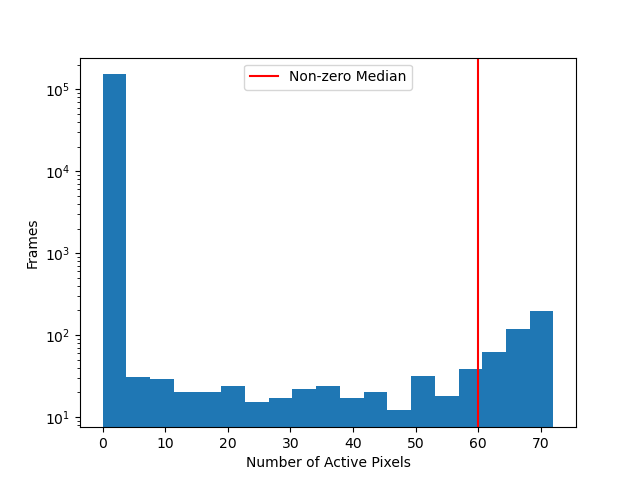
\includegraphics[width=\textwidth]{resources/methodology/active_pixels_dist.png}
        \caption{Without empty pattern.}
        \label{fig:num_active_pixels_cell}
    \end{subfigure}%
    \begin{subfigure}[t]{0.5\textwidth}
        \centering
        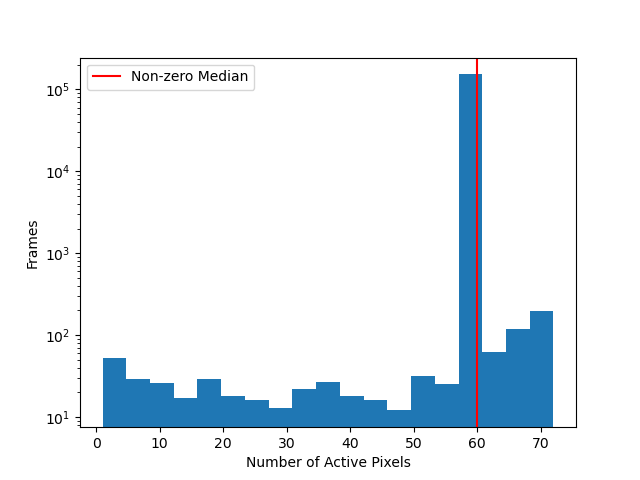
\includegraphics[width=\textwidth]{resources/methodology/active_pixels_dist2.png}
        \caption{With empty pattern.}
        \label{fig:num_active_pixels_cell2}
    \end{subfigure}
    \caption{Distribution of number of active pixels within a cell of size $12\times 12$, it can also be observed that it would benefit from having a minimum sparsity requirement.}
    \label{fig:test}
\end{figure}


With a carefully selected empty pattern sparsity, \textbf{the standard deviation of active pixels was lowered from $\mathbf{3.78}$ to $\mathbf{1.88}$}. It is possible to automate this process by developing an algorithm which finds the optimal cell size and empty pattern sparsity which causes the least variation of number of active pixels per cell. This algorithm would be a part of the calibration process.
\begin{figure}[H]
    \centering
    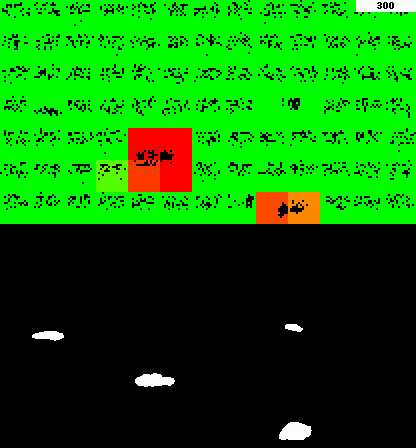
\includegraphics[width=0.7\textwidth]{resources/methodology/htm_grid_output.png}
    \caption{Example Grid \gls*{htm} output and the corresponding input. The color represents the anomaly score for each of the cells, where red means high anomaly score and green means zero anomaly score. Two of the cars are marked as anomalous because they are moving, which is something the Grid \gls*{htm} has not seen before during its 300 frame long lifetime.}
\end{figure}
Since there are now cells that are observing an empty pattern for a lot of the time in sparse data, boosting is recommended to be turned off, otherwise the \gls*{sp} output for the empty cells would change back and forth in order to adjust the active duty cycle.
\subsection{Stabilizing Anomaly Output}
\begin{figure}[H]
    \centering
    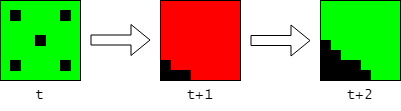
\includegraphics[width=0.7\textwidth]{resources/methodology/empty_to_notempty.png}
    \caption{High anomaly score when an empty cell (represented with an empty pattern with a sparsity value of 5) changes to being not empty, as something enters the cell.}
    \label{fig:empty_to_notempty}
\end{figure}
Another issue with the grid based approach is when a car first comes into a cell. The \gls*{tm} in that cell has no way of knowing that a car is about to enter, since it does not see outside its own cell, and therefore the first frame that a car enters a cell will cause a high anomaly output (\autoref{fig:empty_to_notempty}). This causes the anomaly output to needlessly fluctuate. The band-aid solution is to ignore the anomaly score for the frame during which the cell goes from being empty to being not empty (\autoref{fig:empty_to_notempty_fixed}).
\begin{figure}[H]
    \centering
    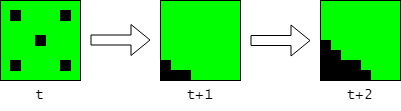
\includegraphics[width=0.7\textwidth]{resources/methodology/empty_to_notempty_fixed.png}
    \caption{In this case, the anomaly score is ignored (set to 0) for the frame in which the cell changes state from empty to not empty.}
    \label{fig:empty_to_notempty_fixed}
\end{figure}
A more proper solution could be to allow the \gls*{tm} to grow synapses to the TMs in the neighboring cells, but this is not documented in any research papers and might also hinder invariance.
\subsection{Multistep Temporal Patterns}
Since the \gls*{tm} can only grow segments to cells that were active in the previous timestep, as was mentioned in \autoref{sec:temporal_memory}, it will struggle to learn temporal patterns across multiple timesteps. This is especially evident in high framerate videos, where an object in motion has a similar representation at timestep $t$ and $t+1$, as an object standing still.
\begin{figure}[H]
    \centering
    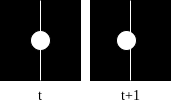
\includegraphics[width=0.3\textwidth]{resources/methodology/high_fps_moving.png}
    \unskip\ \vrule\
    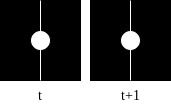
\includegraphics[width=0.3\textwidth]{resources/methodology/high_fps_still.png}
    \caption{Comparison of a moving object (left) and a still object (right)in a high framerate video. They are very similar and could actually end up being represented identically by the SP.}
\end{figure}
This could cause situations where an object that is supposed to be moving, suddenly stands still, yet the \gls*{tm} will not mark it as an anomaly due to it being stuck in a contextual loop. A contextual loop is when one of the predictions at $t$ becomes true at $t+1$, and then one of the predictions at $t+1$ is almost identical to the state at $t$, which becomes true if the object is not moving, causing the \gls*{tm} to enter the same state that it was in at $t$.
\begin{figure}[H]
    \centering
    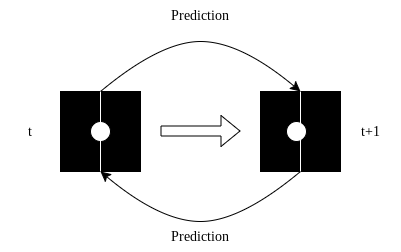
\includegraphics[width=0.7\textwidth]{resources/methodology/contextual_loop.png}
    \caption{Example of a contextual loop.}
\end{figure}
A solution is to concatenate the past $n$ \gls*{sp} outputs as input into the TM, which is made possible by keeping a buffer of past \gls*{sp} outputs and shifting its contents out as new \gls*{sp} outputs are inserted. This follows the core idea behind encoding time in addition to the data, which makes time act as a contextual anchor. However, in this case there are no timestamps that are suitable to be used as contextual anchors, so as a replacement, the past observations are encoded instead.
\par

\begin{figure}[H]
    \centering
    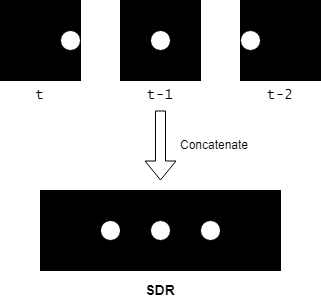
\includegraphics[width=0.45\textwidth]{resources/methodology/temporal_concatenation.png}
    \unskip\ \vrule\
    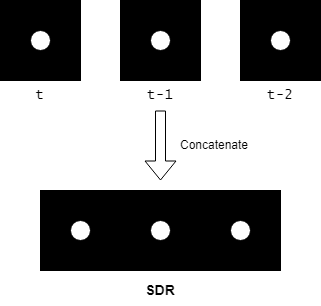
\includegraphics[width=0.45\textwidth]{resources/methodology/temporal_concatenation_still.png}
    \caption{Example of concatenation with $n=3$ when an object is moving from left to right, compared to when an object is not in motion. It can be observed that the SDRs are vastly different.}
\end{figure}
This will force the \gls*{tm} input, for when an object is in motion and when an object is still, to be unique. High framerate videos can benefit the most from this, and the effect will be more pronounced for higher values of $n$. One could feed the past $n$ encoder outputs into the \gls*{sp} instead, but this will lead to a much higher computational requirement, as well as force the \gls*{tm} parameters to be dependent on $n$.
\par
Adding support for multistep temporal patterns to the method used by \textcite{MotionAnomalyDetection}, which is mentioned in \autoref{sec:htm_perf}, could improve their results.
\section{Use Cases}
The most intuitive use case is to use Grid \gls*{htm} for semi-active surveillance, where personnel only have to look at segments containing anomalies, leading to drastically increased efficiency.
\par
One example is making it possible to have an entire city be monitored by a few people. This is made possible by making it so that people only have to look at segments that the Grid \gls*{htm} has found anomalous, which is what drastically lowers the manpower requirement for active monitoring of the entire city.
\section{Summary}
